\section{Respostas de Gustavo Rodrigues dos Santos\label{tarefa-gutorsantos-tarefa-5-1}}

\subsection{A computação é uma atividade científica?}

Com base nas discussões \ref{chap:gutorsantos:impressoes-cienci} e apoiado nas aulas e documentos (\ref{fundamentos:ce}) fornecidos pelo professor, neste breve ensaio, tentaremos responder à pergunta ``A computação é uma atividade científica?''. Portanto devemos definir alguns outros conceitos e guiar e enriquecer a análise da formulação da resposta.

\begin{quote}
Definir o que é uma atividade científica;

Definir o que é computação;

Analisar se a definição de computação sem enquadra na definição de atividade científica. 
\end{quote}

\subsubsection{O que é uma atividade científica?} 

Como visto em \cite{fernandes_consideracoes_2021}, vemos que a produção do conhecimento científico deve ser pautada em alguns princípios para que os resultados obtidos possam garantir uma confiabilidade e veracidade acerca do estudo. Portanto, ao longo da história da humanidade e da ciência, foi desenvolvido o \gls{MetodoCientifico} para garantir a execução de alguns desses princípios, sendo o mais evidente, o princípio da Reprodutibilidade.

Nesse sentido, a atividade científica é a manifestação da produção do conhecimento. Ou seja, a interação, dentro da rede complexa da academia, entre alunos, professores, pesquisadores, instituições e organizações de publicação configuram essencialmente a atividade científica a medida que promovem a manutenção do ciclo da produção do conhecimento. Cada entidade nessa complexa rede possui suas devidas atribuições para a continuidade do ciclo. 

Existem os alunos, que renovam o pensamento dentro do meio acadêmico e consomem os estudos de outros cientistas. Estes são, por sua vez, orientados pelos professores e pesquisadores que além disso, fornecem estudos a serem utilizados como referência teórica pelos recém-chegados bem como por outros pesquisadores. Logo, esses pesquisadores devem estar localizados dentro de um contexto que permita o ``fazer ciência'', diante disso, são as instituições que fornecem este ambiente próprio para a condução das pesquisas, sendo por possuírem bons ambientes físicos de trabalho quanto pelo financiamento de capital para a execução dos estudos. Por fim, o conhecimento deve ser propagado --- seguindo o princípio da publicidade ---  e então as organizações de publicação ao disponibilizar o conhecimento, em meios de comunicação, para que este seja consumido por diversos outros cientistas ao redor do mundo, cumprem este papel e, consequentemente, evita-se que o conhecimento fique restrito apenas à bolha de um certa instituição. Incontestavelmente, existem outros agentes que influenciam nesse ciclo, como os governos e empresas privadas, no entanto, este exemplo ilustra bem o cerne da atividade científica.



Uma atividade científica é aquela que está circunscrita ao ciclo de produção do conhecimento científico. Segundo \cite[p.2]{barton_graphical_1999}, são quatro as fases de um ciclo de produção do conhecimento científico, ilustradas na figura \ref{fig:ciclo:barton}:
\begin{enumerate}
    \item ideação ou hipotetização; 
    \item  planejamento de experimentação;
    \item  experimentação;
    \item Análise dos dados (empíricos).
\end{enumerate}

\begin{figure}
    \centering
    \includegraphics[page=31,clip=true,width=\textwidth]{3-Computacao-Experimental/aulas/3.1-Componentes-Experimento/slides-experimentos.pdf}
    \caption{Ciclo do processo de investigação científica. Fonte: \cite{barton_graphical_1999}\label{fig:ciclo:barton}}
\end{figure}

\subsubsection{O que é a computação?}
A computação, entendida como sendo igual ao processamento de dados, é a ação feita pelos computadores, que envolve o processamento de dados de entrada, gerando dados de saída.

A computação, segundo essa definição estrita, ou seja \textit{strictu sensu}, não seguiria o ciclo de atividade científica, e portanto, não poderia ser considerada uma atividade científica, ou de produção de conhecimento, pois não está em busca da verdade.

Entretanto, a computação que é efetiva precisa sempre processar dados que serão utilizados ou interpretados por algo externo ao computador.
Assim sendo, a atividade de computação é uma ação eminentemente empírica, isso é, produz dados, para uma finalidade qualquer, coerente com a realidade que foi antecipada ou planejada por alguém, o idealizador do programa e o codificador do computador.

Embora não seja uma atividade científica \textit{strictu sensu}, a computação, de forma \textit{lato sensu}, precisa estar inserida em um ciclo produtivo de geração de dados que terão utilidade prática para alguém, sendo dessa forma aproximadamente equivalente a uma atividade de experimentação, no sentido expresso por Barton.

Se considerarmos as ações humanas  antecedentes e sucessoras à computação, elas também apresentam congruência com as demais fases do ciclo de investigação científica, como demonstrado a seguir.

\begin{itemize}
    \item Toda computação
é precedida por um ato criativo de ideação ou formulação de hipóteses feitas por seres humanos, acerca da possibilidade de se criar uma computação que produza um efeito prático desejado junto aos seus usuários. Essa ideação ou formulação, que não precisa ser feita por programadores, visa a produção futura de algum conhecimento novo, ou seja, almeja aproximar-se de alguma verdade. Logo, chega-se à seguinte proposição:
\textbf{
\begin{quote}
    Ideação de um modelo computacional útil e empírico $\cong$ Ideação ou hipotetização científica
\end{quote}
}
\item Uma vez concebidas ideias ou hipóteses sobre um uso útil de uma computação de uma determinada natureza, faz-se necessário o desenvolvimento de um código ou modelo formal, materializado na forma de programas de computador, \textit{firmware} ou hardware, que nada mais é que um plano de execução de um processamento de dados. Assim sendo, pode-se fazer a seguinte proposição:

\textbf{
\begin{quote}
    Codificar  software/firmware/hardware $\cong$ Parte do planejamento de uma experimentação
\end{quote}
}

\item uma vez desenvolvido o modelo computacional, o seu teste em um sistema computacional real ocorre por interação do computador, que opera o modelo, com entidades externas ao computador, chamadas de testadores, que vão trocar dados entre si. O \textit{output} computacional é uma fonte de dados empíricos, similar à ação de experimentação.
O planejamento dos vários casos de teste, para validação do modelo, equivale à ação de controle das variáveis de um experimento científico. Logo, é coerente a proposição a seguir:
\textbf{
\begin{quote}
    Teste sistemático de um sistema computacional $\cong$ Parte do planejamento e execução de experimentos
\end{quote}
}

\item Por fim, concluída a experimentação, os dados empíricos gerados no \textit{output} são analisados e interpretados pelos usuários finais, ou por quem os representa, 
que usarão o computador com o objetivo de analisar se há coerência efetiva entre a realidade externa ao computador, com a ``realidade'' expressa pelo modelo computacional, na produção de \textit{outputs} coerentes com os \textit{inputs} recebidos.
Ou seja, as ações de uso do sistema computacional produzido de forma metodicamente organizada nas etapas anteriores, equivalem a uma ação sistemática de aquisição de novo conhecimento. Em última instância, o novo conhecimento é útil se o usuário fica ``feliz'', se o sistema computacional é coerente, preciso, de boa usabilidade, flexibilidade etc. Concluí-se com a seguinte proposição:
\textbf{
\begin{quote}
 Uso de um sistema de computação $\cong$ Análise dos dados (empíricos)    
\end{quote}
}
\end{itemize}

Depreende-se, pelos argumentos expostos, que a computação, \textit{lato sensu}, é uma atividade que se aproxima bastante da atividade científica.

\subsection{A computação é uma ciência experimental? Justifique. }

Com base nos argumentos anteriores, a computação \textit{lato sensu}, quando usada no sentido de ideação, codificação, teste e uso de computadores aproxima-se da produção do conhecimento científico pelo método experimental.

\subsection{A computação é uma ciência empírica? Justifique. }

Com base nos argumentos anteriores, a computação \textit{lato sensu}, quando usada no sentido de ideação, codificação, teste e uso de computadores aproxima-se da produção do conhecimento científico baseado no consumo e geração de dados, sendo assim, uma atividade eminentemente empírica.



